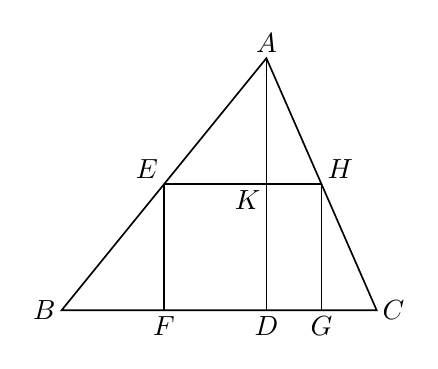
\begin{tikzpicture}[x=1cm,y=1cm,font=\normalsize,
 geometry edge/.style={solid,line width=.6pt},
 geometry mark/.style={solid,line width=.6pt},
 geometry label/.style={font=\normalsize,inner sep=2pt}]
\coordinate (A) at (2.6,3.2);
\coordinate (B) at (0,0);
\coordinate (C) at (4,0);
\coordinate (D) at (2.6,0);
\coordinate (E) at (1.3,1.6);
\coordinate (H) at (3.3,1.6);
\coordinate (F) at (1.3,0);
\coordinate (G) at (3.3,0);
\coordinate (K) at (2.6,1.6);
\draw[geometry edge] (A)--(B)--(C)--cycle;
\draw[geometry edge] (A)--(D);
\draw[geometry edge] (E)--(H);
\draw[geometry edge] (E)--(F);
\draw[geometry edge] (H)--(G);
\node[geometry label,above] at (A) {$A$};
\node[geometry label,left] at (B) {$B$};
\node[geometry label,right] at (C) {$C$};
\node[geometry label,below] at (D) {$D$};
\node[geometry label,above left] at (E) {$E$};
\node[geometry label,above right] at (H) {$H$};
\node[geometry label,below] at (F) {$F$};
\node[geometry label,below] at (G) {$G$};
\node[geometry label,below left] at (K) {$K$};
\end{tikzpicture}
